We begin this chapter with a look at related work in the field of artificial intelligence: approaches, architectures, implementations, and philosophies on which later parts of the thesis draw. After that, in Section~\ref{sec:preliminaryConsiderations}, we will go through biological and neurological considerations that shall ground the models and architectures proposed herein. Lastly, Section~\ref{sec:whiteBoxModel1} will outline a white-box model of cognition which assumes various parts of a central nervous system observing and influencing each other relatively freely. We specifically contrast this with the black-box model of structured programming, where the inner workings of functions and procedures are oblique to the caller.

\section{Related Work}

\paragraph{Cognitive architectures.} This thesis falls into the category of cognitive architectures and the integrated approach to AI, pioneered by people like Rodney Brooks and his subsumption architecture, and \cite{brooksSubsumption}, Douglas Hofstaedter, who famously wrote about many aspects of AI in Gödel, Escher, Bach \cite{geb}, and who created the Copycat analogy-making program \cite{copycat}. Another important work is the Hierarchical Control System of James Albus \cite{albusHCS}, in which cognitive tasks are organized hierarchically and delegated by nodes on higher levels to those on lower ones (this is similar to the mesh-like organisation of components described in Section~\ref{sec:mathematicalModel}, and to the layered structure of Minsky's {\em The Emotion Machine} \cite{emotionMachine}). The organisation described by Albus \cite{albus93areference} is, moreover, very similar to the one in Section~\ref{sec:proposedArchitecture}, with world simulator, belief generator, sensory perception, and knowledge base (herein called ``memory'') modules being mostly analogous. Another large and notionally similar system is Carnegie-Mellon's 4CAPS \cite{4caps}, which posits small, relatively simple components, individually doing simple tasks, and having only limited computational resources. Most of 4CAPS's stated principles can be recognized in the coming sections \cite[Operating Principles of 4CAPS]{4caps}:
\begin{quote}
	\begin{enumerate}
		\setcounter{enumi}{-1}
		\item Thinking is the product of the concurrent activity of multiple brain areas that collaborate in a large-scale cortical network. \ellipses
		\item Each cortical area can perform multiple cognitive functions, and conversely, many cognitive functions can be performed by more than one area.
		\item Each cortical area has a limited capacity of computational resources, constraining its activity.
		\item The topology of a large-scale cortical network changes dynamically during cognition, adapting itself to the resource limitations of different cortical areas and to the functional demands of the task at hand.
		\item The communications infrastructure that supports collaborative processing is also subject to resource constraints, construed here as bandwidth limitations.
	\end{enumerate}
	
	\quad\quad\ \ellipses
\end{quote}

The probably earliest example of a cognitive architecture was Allen Newell's and Herbert~A.~Simon's {\em Logic Theorist}, created in 1955 \cite[p. 44]{crevier93}. Simon's theory of bounded rationality \cite{Gigerenzer2001} --- the idea of finding a merely satisfactory solution instead of a (provably) optimal one --- is very similar to the loop between belief generation and evaluation described in Section~\ref{sec:implementation}. In both cases, agents with limited information search heuristically for the first solution that they find acceptable. Unlike exhaustive search methods (e.g. A*), this does not guarantee the best possible results, but it is much more cost-effective and closer to the way real humans solve problems. In spirit, this is also similar to the {\em Procedural Reasoning System} of Michael Georgeff et al. \cite{pcs}, which is based on the belief-desire-intention model \cite{Rao95bdiagents, Bratman87}. Much theoretical work has been done on BDI, but it is only tangentially related to this thesis.

\paragraph{Sloman.} Many of the fundamental ideas in this thesis can be found in Alan Sloman's works \cite{sloman1993, sloman1997, sloman1999, sloman2000, slomanSimAgent}, especially in {\em Beyond shallow models of emotion}. Therein, he formulated the crtierion of evolvability in the context of cognitive architectures and postulated the possibility that nervous systems may be chaotic (but not unorganized). The agent architecture in Section~\ref{sec:implementation} substantially resembles his, though it was not taken from there. The similarity is, however, indicative of a great deal of shared thought.

\paragraph{Implementation.} In terms of software engineering, our model has similarities, both to the Actor model \cite{hewittActor}, and to publish/subscribe architectures \cite{publishSubscribe} --- although more as a concession to practicality and less because of a similarity to their theories. The theoretical basis of our implementation is the postulate that the components of the brain function as white boxes and that other components may listen in on their activity, so to speak. Since this is diametrically opposed to the traditional idea of the procedure/function as a black box, which nigh every programming language follows, we compromise and model the cognitive structure as a mesh of loosely coupled components communicating via passing. This description is reminiscent to the Actor model developed by Carl Hewitt et al. , although there are differences\footnote{Although we do not describe the implementation in the language of the Actor model, a translation into it would be quite easy. Such a translation would require using only very rudimentary features of the model, however, and, as that is not the focus, we forego the task.}: in the Actor model, the topology of the network may change through the creation of new actors, and messages are always passed from one source to known targets (via addresses). In our model, on the other hand, there is no topology in a strict sense; messages are put into a global message storage and every component is free to consume any message it deems relevant. Senders do not know who will read their output, and consumers do not know the sources. This arrangement can be seen as a particularly loose variant of a publish/subscribe architecture, in which the source and the target of a message are completely unaware of each other, and in which there are no specific channels to which one may subscribe. The only criterion by which messages may be accepted or rejected is their content.

% We also make use of already existing solutions --- specifically answer-set programming and the \acthex\ solver \dlvhex. The internal world simulation of our agents makes use of the non-monotonic reasoning provided by ASP and \acthex.  Answer-set programming was created by Gelfond and Lifschitz \cite{asp1}. Soon after them, Subrahmanian made the connection between ASP and planning \cite{Subrahmanian95relatingstable}. Together with Eiter and others, he later developed the \acthex\ language which allowed provided a framework for decision making in logic programming via external input and output atoms \cite{heterogeneous1, heterogeneous2, heterogeneous3}.

\paragraph{Nouvelle AI.} Lastly, the overall goal, if not the method, of this thesis echoes that of the {\em nouvelle AI} of, again, Brooks, who claims that
\begin{quotation}
	the Von Neumann model of computation has lead Artificial Intelligence in particular directions. Intelligence in biological systems is completely different. \cite{Brooks91intelligencewithout}
\end{quotation}
The nouvelle AI approach stands in contrast to traditional AI in that it does not aim for human-level performance at specific tasks, but rather for the faithful reproduction of the behaviour of lower animals like dogs \cite{nouvelleAI}. Brooks might be closer to the biological realities in his desire to abandon the von Neumann model in favour of biologically modelled computation, though we will only take only general inspiration from his approach, not follow it closely. As our goal is merely a proof-of-concept implementation, and since the realization of truly novel programming, biologically oriented, paradigms is quite laborious, we opted for a compromise position and only tried to imitate biological computation in general spirit rather than in every detail.

\section{Preliminary Biological Considerations}\label{sec:preliminaryConsiderations}

In this section, we will go over the foundational ideas that, while serviceable on their own, will underlie the work in the second part of this work. The information will primarily concern biology, computational models, and the brain as a product of evolution. Biologists will find all of it terribly basic, but this document is not intended for them; it is intended for computer scientists --- who, I feel, have not truly taken to heart the consequences of the routes our nervous systems have taken through history for their present state. Sure enough, we have things {\em called} ``evolutionary algorithms'' and ``machine learning'', but names such as these invite us to a perilous confusion of labels with the real things. Inspired though such mathematical abstractions may be by biological processes, they are not the equivalents of these processes. Re-creating the end-products of biology demands an understanding of biology on its own terms, not through the lens of misguidingly named mathematical abstractions. Providing the basis of such an understanding will be our aim for the next couple of pages.

\paragraph{Historical and designed artifacts.} In order to understand how our brain works or could work, we must possess conceptual clarity --- we must conceive of it, not as a product of one-time engineering, but as a historical artefact. Unlike ``perfect'' systems, like Peano arithmetic and the $\lambda$ calculus, those which grew historically does not make sense if one only looks at their current snapshot. One will find nonsensical solutions, and attempts to mitigate the consequences of earlier designs that have now become disadvantageous. The system as a whole might, at first glance, appear incomprehensibly and needlessly complicated. Of all such systems, the human brain might well be the most complex one; the task of understanding it correspondingly harrowing. Sloman asked whether the the brain might have no architecture at all  \cite[p. 5]{sloman1997}:

\begin{emquote}
	Another question on which there is disagreement is whether the provision of a large set of capabilities, such as those listed above, necessarily involves the creation of an {\em intelligible} design, with identifiable components performing separate tasks, or whether the functionality could sometimes (or always?) emerge only in a very complex and incomprehensible fashion from myriad interacting components.
	
	For example, experimenters using genetic algorithms to evolve neural sets to control a robot sometimes create networks that work, but which seem to be impossible to understand (not unlike some legacy software which has grown over many years of undisciplined developments).
\end{emquote}

It the classical sense, it probably does not, but we ought to be cognizant that ``the classical sense'' was induced by tradition and the limits of human cognitive ability. We might dismissively describe the brain as a jumbled, tangled chaos of neurons, but the fact that we do not recognize a structure by no means implies that one does not exist. Things, contrary to what is oft espoused, do not ``just work''; if they reliably produce complex results, they must have an architecture inside them, independent of our ability to recognize or understand it as such. We merely need to relax the notion of ``architecture'' to include structures that result from incremental change and the creative combination of pre-existing parts. While the results of such processes are often extremely unintuitive and often even incomprehensible to us, we at least have a way of understanding them by re-tracing their evolution. Doing so is laborious and requires a huge amount of data (which we currently do not have), but this approach of regarding brain function as through-and-through Darwinian (as opposed to having been pieced together) might bear results that have, so far, eluded the other schools of thought in the field.

What, one might now ask, is the consequence of such a view? The first is that each new feature in the developmental history had to have been useful on its own. The second is that it allows the distinction between what I will herein call \textsc{efficient} systems and \textsc{clean} systems. Since, at each stage of its evolution, the organism that carried the brain had to be viable, the end product is by definition guaranteed to be ``efficient''. Because of that same fact, however, it is all but guaranteed not to be ``clean'': for one, it was not possible to snap whole new components into the system; it would have also been impossible to combine old components in the elaborate and precise ways in which a human engineer might use parts. Worse, old components were almost certainly not discarded when new and better ones came into being. A good exposition of this process in humans can be found in Paul MacLean's seminal work {\em The Triune Brain in Evolution} \cite{maclean1990}.

\begin{figure}[!h]
	\centering
	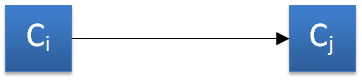
\includegraphics{Figs/noNervousSystem.png}
	\caption{Relationship between the components of an organism without a nervous system.}
	\label{fig:noNervousSystem}
\end{figure}
%\vspace{-0.18cm}
\subsection{Origin of Nervous Systems} The evolution of nervous systems in organisms dates back to the development of primitive electrical signalling in eukaryotes, using calcium action potentials\footnote{See any textbook on evolutionary biology.} and sodium channels \cite{Liebeskind31052011}:

\begin{emquote}
	Voltage-dependent sodium channels are believed to have evolved from calcium channels at the origin of the nervous system.
\end{emquote}

These sodium channels predated modern-day neurons, but served the same fundamental purpose of acting as control systems. We can readily conceive the benefits of imparting a control system onto an organism with the following thought experiment: let us imagine a microscopic organism without any sort of nervous system --- all of its behaviour is hard-coded and mechanical. It can take in nutrients through its cell walls or through an opening; parts of it can contract or expand in response to stimuli like light or pressure; homeostatic conditions can influence its chemistry. Figure~\ref{fig:noNervousSystem} shows this schema: if we enumerate the constituent parts or {\em components} of an organism as $\{C_1,\dots,C_n\}$, the organism's behavior is caused by signals being sent between $C_i$ and $C_j$ (the case $i=j$ is possible). Such an organism suffers from three disadvantages: (a) reactions are localized, as two of its components might be too far apart to communicate in a timely manner or at all; (b) its repertoire of behaviours is necessarily simple and (c) it is not very adaptable.

Precursors to nervous systems ameliorated (a) first via action potentials, which were intracellular electrical signals \cite{Liebeskind31052011} (emphasis mine):
\begin{emquote}
Another key animal innovation was the nervous system, which is present in all but a few animals (i.e., sponges and placozoans). {\em Rapid, specific, long-distance communication among excitable cells} is achieved in bilaterian animals and a few jellyfish (cnidarians) through the use of action potentials (APs) in neurons generated by voltage-dependent sodium (Na$_\mathrm{v}$) channels. Voltage dependent calcium (Ca$_\mathrm{v}$) channels evolved in single-celled eukaryotes and were used for intracellular signaling. {\em It has been hypothesized that Na$_v$ channels were derived from Ca$_v$ channels at the origin of the nervous system} \textsf{[the results in the paper support the hypothesis]} (3), thereby conferring the ability to conduct action potentials without interfering with intracellular calcium. This view was reinforced by the apparent lack of sodium currents in sponges (4).
\end{emquote}

The introduction of dedicated, long-distance\footnote{The term ``long-distance'' may very well mean ``long-distance within a single cell''. Franti\v{s}ek and Mancuso argue in {\em Deep evolutionary origins of neurobiology: Turning the essence of ``neural'' upside-down} \cite{frantisek} that neural analogues already existed in prokaryotes (bacteria and archaea; organisms without cell walls and nuclei) and unicellular eukaryotes.} signalling cells between parts of an organism created the possibility of not only transmitting, but also modifying information. The moment an organism's parts do not communicate directly biochemically/mechanically, but over transmissions lines, evolutionary processes acting upon these lines are able to mutate them so that they change the signals. The first changes might consist of amplifying, diminishing, or distributing signals. Over time, the nerves may come to act as transducers on the stream of signals; in some rudimentary sense, they may begin to compute functions. Schematically, we see this in Figure~\ref{fig:nervousSystem}, where a function $F$ is interposed between two components. Not all components of an organism are created equal, of course. The first and most important use of nerve cells was the communication between sensory organs and the movement apparatus of the organism, and the bulk of nerve cells were located close to the sensory organs, where they processed information. A mere handful of neurons are not able to compute much, but they must have conferred considerable advantage to their owners.

\begin{figure}
	\centering
	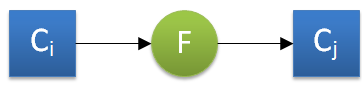
\includegraphics{Figs/nervousSystem.png}
	\caption{Relationship between the components of an organism possessing a nervous system. $F$ can be understood as a simple signal transformer or a central coordinating mechanism.}
	\label{fig:nervousSystem}
\end{figure}

The history of these developments is not entirely clear, but action potentials are present in all animals (with the exception of sponges) and in plants \cite{Leys01051999, PCE:PCE1614}. 
A step up from mere stream transducers are the nerve nets that permeate the entire bodies of cnedaria (jellyfish) and the nerve cords that run along the bodies of bilateria (animals with left and right sides). In Figures~\ref{fig:animalia2} and \ref{fig:animalia} we see them in the phylogeny of the kingdom animalia. Both can process signals in a sophisticated way, and enable the performing of varieties of complex tasks, although the sets vary widely from species to species.

\begin{figure}
	\centering
	\begin{subfigure}[t]{0.30\textwidth}
		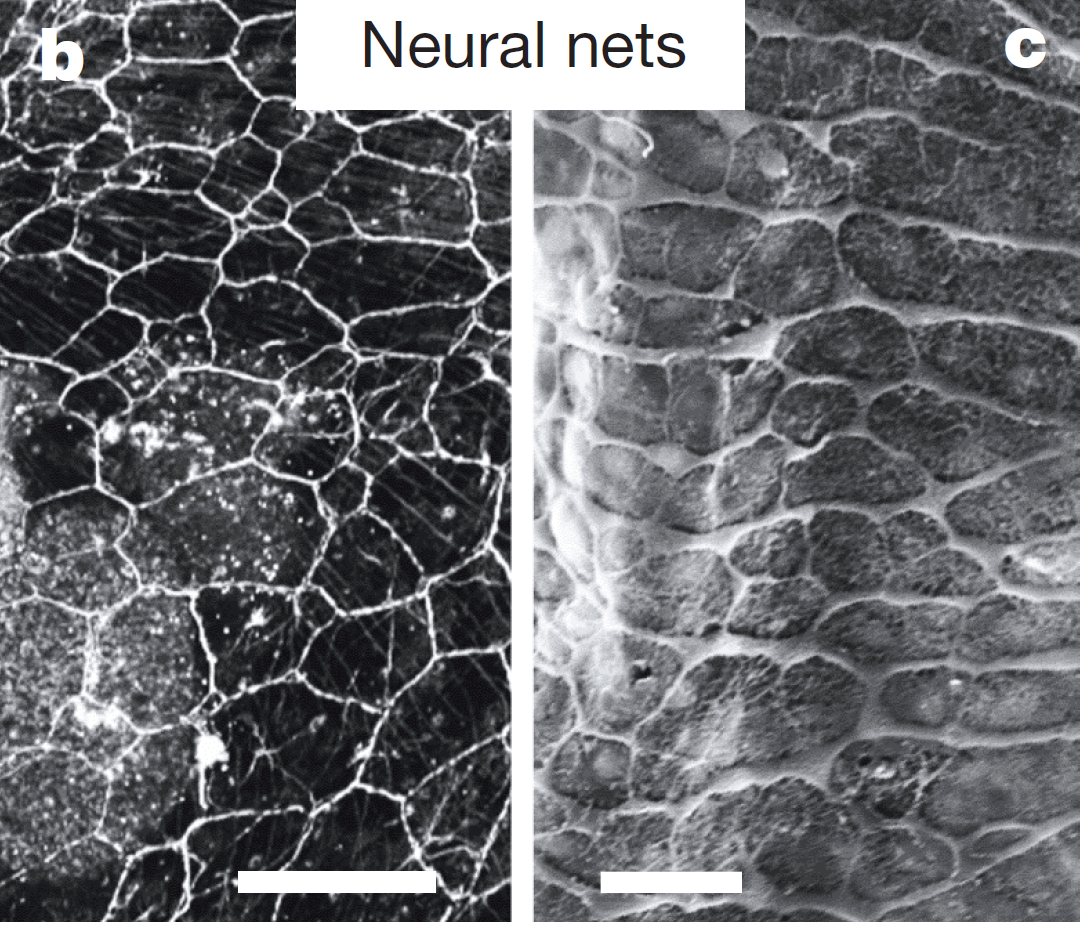
\includegraphics[width=\textwidth]{Figs/neuralNet.png}
		\caption{Nerve nets in ctenaphora.}
		\label{fig:nerveNets}
	\end{subfigure}
	\begin{subfigure}[t]{0.65\textwidth}
		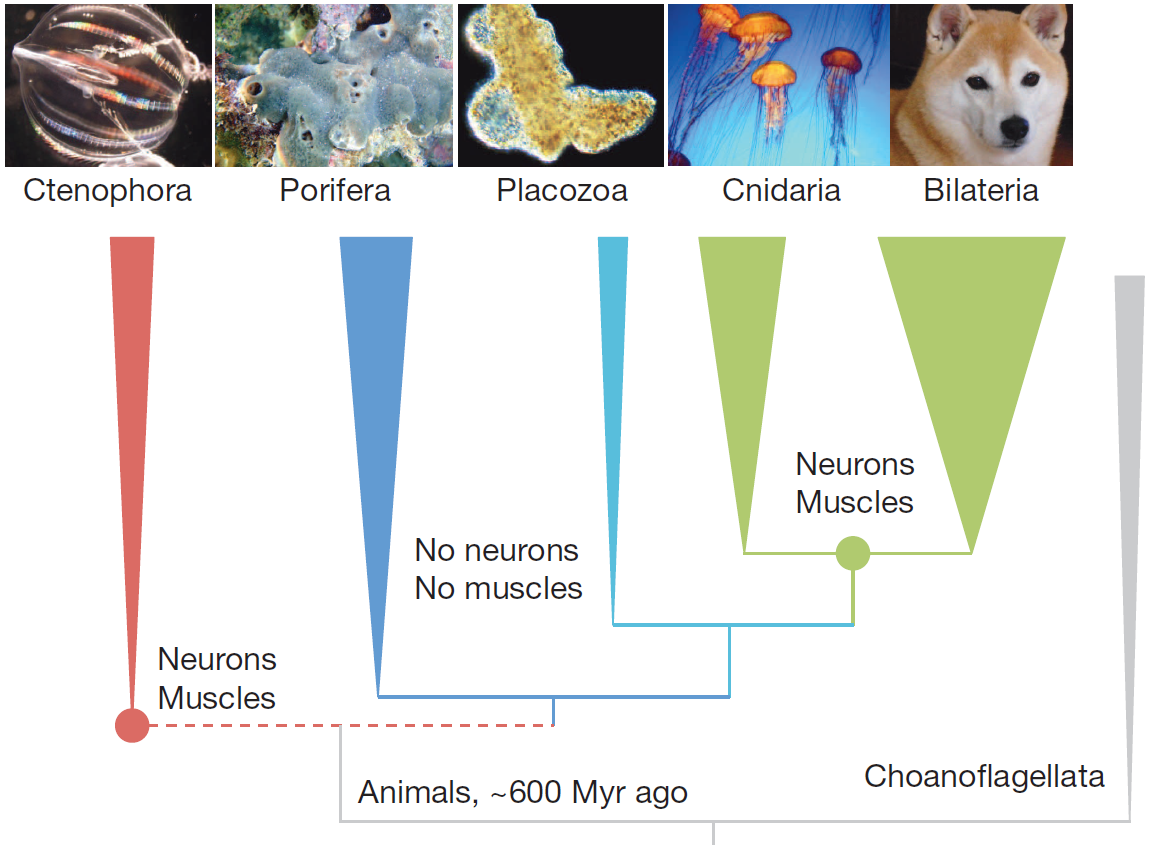
\includegraphics[width=\textwidth]{Figs/animalia3.png}
		\caption{Phyolgeny of the animalia. Even Ctenophores, macroscopic marine invertebrates which predate both jellyfish and bilateria, have nervous systems in the form of distributed nerve nets.}
		\label{fig:animalia2}
	\end{subfigure}
	\caption{Nevre nets and phylogeny of animalia. From {\em {T}he ctenophore genome and the evolutionary origins of neural systems} \cite[p. 100]{animalia2}.}
\end{figure}

\begin{figure}
	\centering
	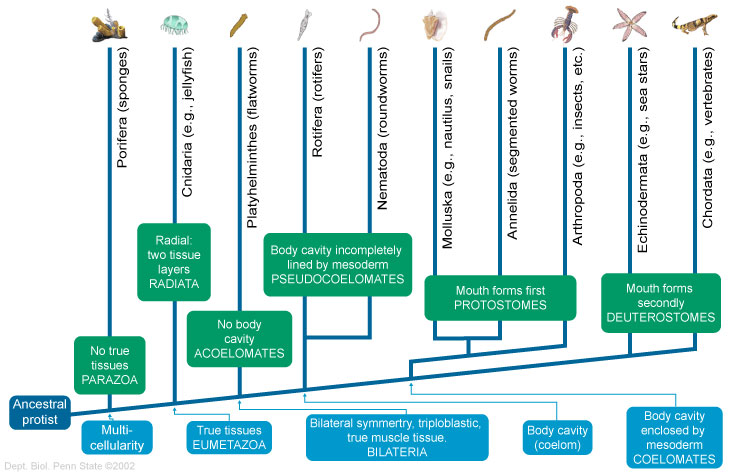
\includegraphics[width=0.8\textwidth]{Figs/animalia.jpg}
	\caption{Phyolgeny of the animalia. Note the cnidaria and bilateria; both of these have types of nervous systems. From {\em Animals I -- An Overview of Phylogeny and Diversity} \cite{animalia}.}
	\label{fig:animalia}
\end{figure}

\begin{figure}
	\centering
	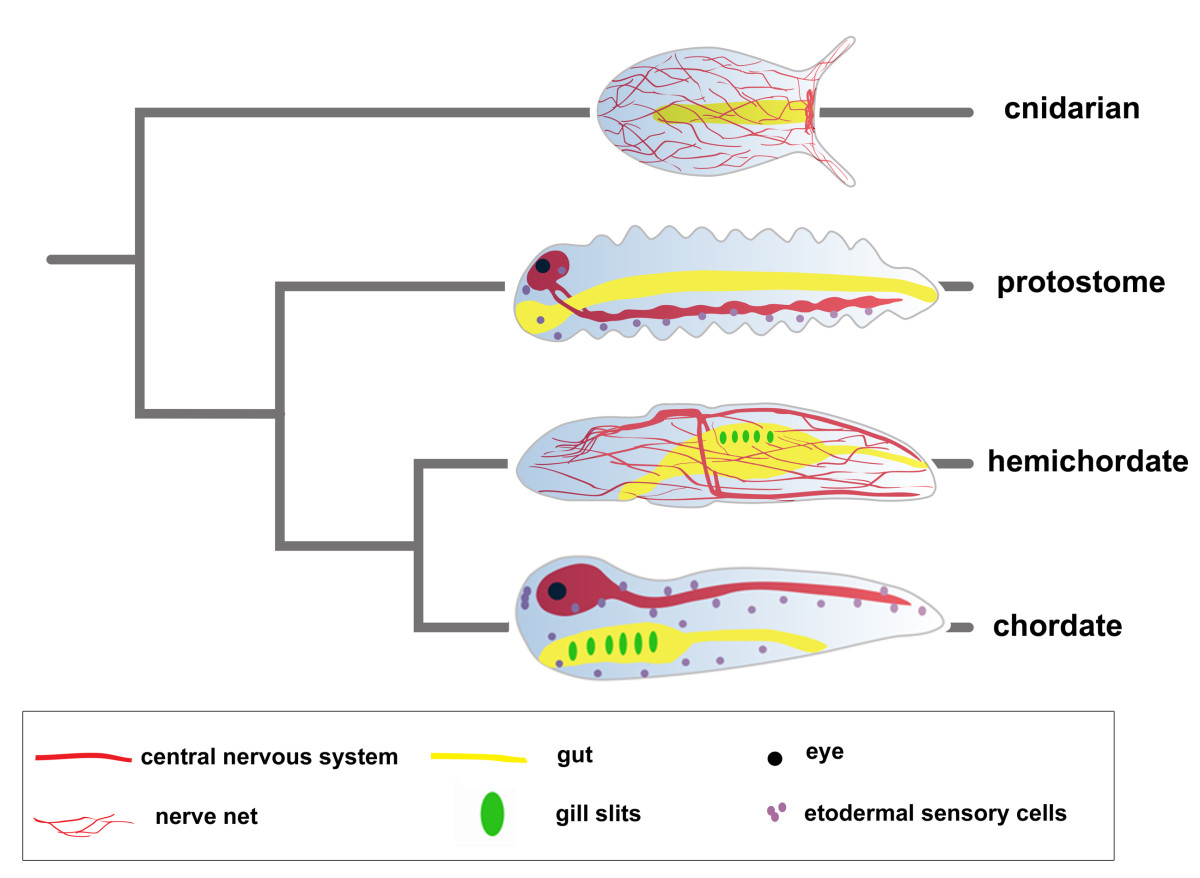
\includegraphics[width=0.8\textwidth]{Figs/chordata.jpg}
	\caption{Body plans for metazoans. The bottom three items are all bilateria and all have nerve cords of some kinds, but only the bottommost (chordates) have a dorsal (upper) nerve cord. Vertebrates are a subphylum of the chordata. From {\em Evolution of bilaterian central nervous systems: a single origin?} \cite[p. 3]{chordata}.}
	\label{fig:chordata}
\end{figure}

\paragraph{Central nerve cord and cephalisation.} Nerve nets, while interesting, are not our aim. Unlike jellyfish, bilateria have a central nerve cord which runs from their front to their back. At various points alongside the cord, we find ganglions --- thickenings containing larger amounts of nerve bundles. In all animals but worms, the frontal ganglion further thickened until it came to contain the overwhelming majority of the organism's neurons --- forming the head. While substantial neural activity was occurring before this time, it is only here that it becomes to proper to speak of brains, and where we can begin to analyse macroscopic structures like lobes.

\begin{figure}
	\centering
	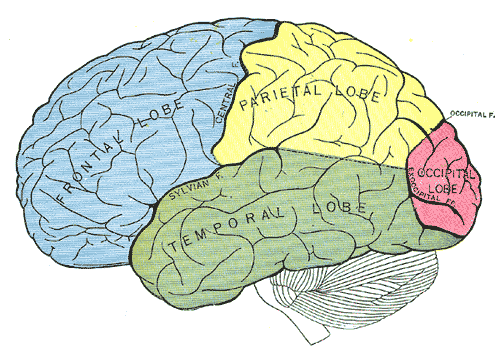
\includegraphics[width=0.65\textwidth]{Figs/brain.png}
	\caption{Illustration of the cerebrum with lobes shown. Hidden: limbic lobe, insular cortex. From {\em Anatomy of the human body} \cite[Fig. 728]{graysAnatomy}.}
	\label{fig:brain}
\end{figure}

Very briefly: vertebrate brains are subdivided into hinbrain, midbrain, and forebrain, having evolved in this order. The forebrain (cerebrum) is responsible for all higher functons and is again divided into six lobes, which we see in Figure~\ref{fig:brain}. The functions performed by these lobes are not precisely understood, but a number can be clearly associated to one lobe. The frontal lobe, for instance, is responsible of conscious thought; the temporal lobe processes auditory and olfactory signals; the occipital lobe deals with sights.\footnote{Interestingly, the occipital lobe is at the {\em back} of the head.} While some functions, like memory, are not neatly localisable, we can nonetheless see in the anatomy of vertebrate and mammalian brains the accruing of large groups of functions: motor control, smell, hearing, sight, reason, emotions. The question of organisation remains, however: it is one thing to say that we have hearing and smell, but what, if anything, ties these experiences together? We, after all, perceive the data from all our senses as one integrated experience. Here, views diverge. The common-sense belief is that we simply have one, indivisible consciousness. Such a view would implicate the frontal lobe as an central organising unit, without which an organism, even if it could smell or see, would not consciously do so. Minsky, Sloman, and Dennett argue persuasively, but speculatively, against this view in their works \cite{emotionMachine,societyOfMind,sloman1991, dennett1991}. They differ on the details, but all agree that the unified consciousness is an illusion; that it is not a single ``I am''-thing gathering raw data, but a dispersed locus of experiences that we merely perceive as immediate.\footnote{Dennett criticises the idea of a \caps{consciousness-thing} with the concept of the ``Cartesian theater'' \cite{dennett1991}. According to him, positing that there is such a thing in our brains, and that it observes all other brain functions, is fundamentally problematic: if there is such a sort of homunculus in our heads that, say, sees the result the output of visual processing in the manner in which one would see a film, then how its visual perception work? Is there yet another a homunculus inside the homunculus that interprets visual information? Such a view implies either an infinite regress, or the algorithmic inexplicability of some part of the brain.} In this view, the frontal lobe, while still instrumental, would not be the only contributor. All other regions of at least the cerebrum would contribute in some way to the organism's conscious experience. An animal without a frontal lobe would not be conscious in the same way as we are, but it would not be utterly blind either --- it would already have some dim awareness of its existence; some rudimentary ``I am'' that we can hardly imagine would already be present in it. To quote Sloman (emphasis mine):\footnote{The quotation appears in {\em The Emotion Machine} \cite[p. 97]{emotionMachine} and Minsky attributes it to a post made by Aaron Sloman in the \texttt{comp.ai.philosophy} newsgroup, but I have been unable to find the original.}
\begin{emquote}
It is not worth asking how to define consciousness, how to explain it, how it evolved, what its function is, etc., {\em because there's no one thing for which all the answers would be the same. Instead, we have many sub-capabilities, for which the answers are different}: e.g., different kinds of perception, learning, knowledge, attention control, self-monitoring, self-control, etc.
\end{emquote}

\paragraph{Implications.} The point in all this is not to give an detailed summary of evolutionary neurobiology; it is to show that nervous systems are ancient, gradually developed things. They have been shaped by the vicissitudes of hundreds of millions of years, and they could have developed in other ways. They were not planned, as a human would understand to word. If we are to gain headway in piecing together the ``big picture'', we must take these facts to heart, and choose our modelling methods accordingly.

In the abstract of this work, I described the biological and the idealistic approaches as being polar opposites, and this is true as far as engineering is concerned, but in terms of their assumptions, false. They are both idealistic. Neural networks, insofar as their users want to re-create human behaviour, implicitly presuppose an intelligence in neurons that is not there. The comparatively small network is taught to compute some desired function, the hope being that it might thereby come to perform some complex, real-world function like common-sense reasoning. In principle, this strategy could work, but in practice, it is unrealistic --- the environment in which real organisms had to succeed was the planet's ecosphere; billions upon billions of nervous systems of all complexities were run over millions of years; nervous systems died off and were re-created from scratch by genes. It is therefore entirely unreasonable to assume that neural network, trained against an objective function over a period of hours or days could re-create the function a biological organism, unless one were to suppose that there is some inherent quality in neurons that strives for such; that groups of cells somehow {\em wish} to organize themselves into specific configurations in which they are able to perform activities we would call ``cognition''. 

All this being said, we should not confuse criticism of the suitability of a method for a specific purpose with criticism of its suitability for any purpose. Neural networks have proven useful in understanding mental activity at small scales; both they and the symbolic/logic-based approaches have had a myriad of industrial applications. From this, however, it does not follow that we can build genuinely intelligent agents with them. Our only means of doing that (the only means that remain) is to laboriously unravel the developmental history of animal brains, step by step, making sense of each development in context. Where empirical data are not available, we at least have to hypothesize how things could plausibly have happened. To day, structural and genetic analyses have been done (via genetic sequencing and MRI), but they do not deliver sufficiently detailed data. Such methods are rather akin to measuring voltages and task time in a PC --- they do tell us something, but an observer would never infer the existence of e.g. compilers, call stacks, or type systems from such observations. For an understanding of the brain so specific that we can re-implement it in a computer, we will need currently non-existent and not-conceived-of technology. Until that day --- and this will be the main thrust of this thesis --- guesswork will have to suffice.

\subsection{Ways of Adaptation}

After the philosophical groundwork and biological basics, let us describe possible means by which nervous systems can change and acquire new features. We begin with the observation that the existence of neuron bundles between parts of an organism is analogous to a loose coupling of components in a software systems. By having intermediaries that take over the task of communication, selection pressure can produce more and more complex functions, since it no longer has to act upon the body parts that send various signals, but change the nervous system that processes these signals instead. As example: pain receptors, muscles fibres, and the optical nerve have been unchanged for quite some time, long pre-dating the human species, but more recent brain developments have given us the ability to utilise them in novel ways --- by providing a rich mental experience of suffering, playing instruments, and mentally rotating objects, respectively. Manipulating the software is far easier and more quickly done than doing so with the hardware, so to speak.

Having said that, the changes still have to have occurred incrementally. Even if a nervous system can change quickly (for evolutionary timescales), it still has change in tiny steps. We shall leave the matter that for the time being, but, as we will discuss later, this simple fact has profound computational consequences that are seldom thematised in discourse on this matter. 

Let us return to the consideration of primitive life forms. We can imagine the malleable neuron bundles of such ancient organisms changing in a variety of ways in the face of selection pressure: when the environment required it, they could, after several generations, start to compute different or more elaborate functions. An organism which had had developed in an environment where food was abundant in bright places and which had now found itself in darkness would have benefited from a variety of plausible changes, such as
\begin{itemize}
	\item an inversion of its light-seeking behaviour,
	\item switching off its metabolism in light places to conserve energy,
	\item accelerating its metabolism in dark places to make better use of the food there.
\end{itemize}

Of course, other changes would have also been possible, such as the metabolization of different food sources,\footnote{A current-day example is given by nylon-eating bacteria, which have developed in the last century and which now have an abundant food source and no competition.} but we can see how the aforementioned three could have been effected through mutations in a simple nervous system. For a system to permit such mutations, it must be far more robust than most products of human engineering, however. If one were to take out a piston in a car or replace a cogwheel in a mechanical clock with a differently sized one, the machine would, in most cases, simply break. In all others, it would catastrophically malfunction. Machines are designed to fit together perfectly and their complexity tends to be irreducible. Even software, which is more readily changed, is easily broken by small-scale tinkering.

When discussing how they can evolve and, in particular, {\em evolve to perform new tasks} and not just variations on old ones, explanations are again constrained by two criteria: (a) the change has to be small, or at least have a small cause\footnote{The effect does not have to be small --- changes in single genes can switch entire components on or off. The MYH16 gene, which is present in non-human primates but has been switched off in humans, is an example. In us, its disabling lead to a drastic reduction in the size of jaw muscles and a corresponding increase in brain size~\cite{carroll2005}. Nonetheless, such events are rare and not the main drivers of evolution.} and (b) each change must be beneficial in the short term.\footnote{Caveats apply: if the selection pressure on a group of organisms is not too strong, changes which may be sub-optimal but perhaps beneficial at some later point may spread, and non-selective processes like genetic drift can also play a role.} Something that we would conventionally recognize as a program, something which has precise notions like "instruction" and "call structure" is probably not suited to this pattern of changes.\footnote{Cf. evolutionary program generation, in which expression trees mutated. I charge that such algorithms are not adequate models of what happened in the evolution of our brains.} Instead, we ought to imagine the brain as a mesh of computation in which functions are computed cumulatively, so that small changes in neural structure only lead to small changes in output.

To illustrate this, we can look at a simple neural network in Figure~\ref{fig:neuralNetwork}, with a marked node $N_x$. Figure~\ref{fig:unlikelyEvolution} shows an unlikely change scenario in which some new component/function is cleanly grafted onto the system. Figures~\ref{fig:likelyEvolution} and \ref{fig:copyEvolution} then show two more likely scenarios: in the first a mutation causes $N_x$ to be split and the new nodes take over some of its connections. In the second, a larger component is accidentally copied as-is and, over time, is moulded to do something useful.\footnote{Such copies can be caused by mutations and are known to happen with some frequency in nature.} In time, new functions can thus grow into the system, but never in the manner in which, say, an engineer would implement a new feature. 

\begin{figure}
	\centering
	\begin{subfigure}[t]{0.45\textwidth}
		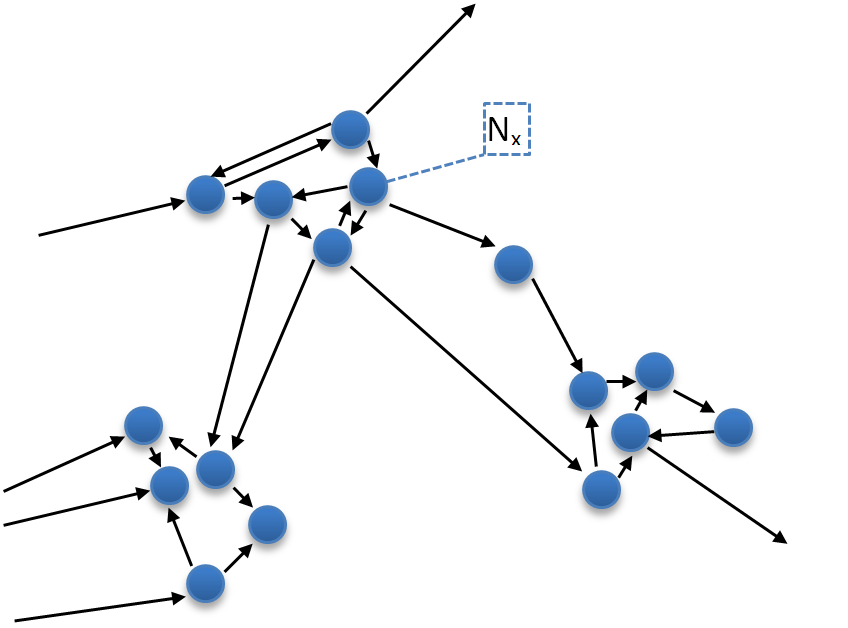
\includegraphics[width=\textwidth]{Figs/neuralNetwork.png}
		\caption{A simple neural network.}
		\label{fig:neuralNetwork}
	\end{subfigure}
	\begin{subfigure}[t]{0.45\textwidth}
		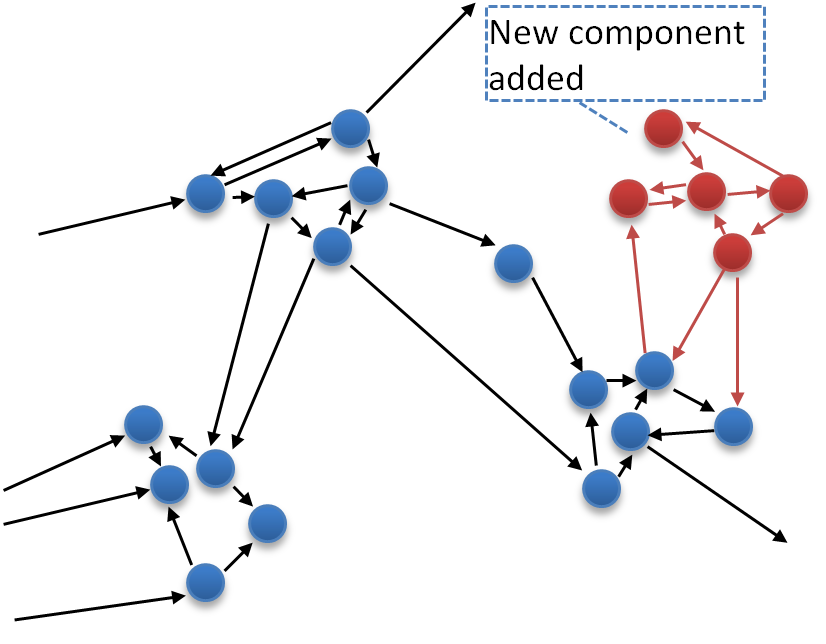
\includegraphics[width=\textwidth]{Figs/unlikelyEvolution.png}
		\caption{An unlikely change scenario in which new, discernible components are grafted on from whole cloth.}
		\label{fig:unlikelyEvolution}
	\end{subfigure}
	\begin{subfigure}[t]{0.45\textwidth}
		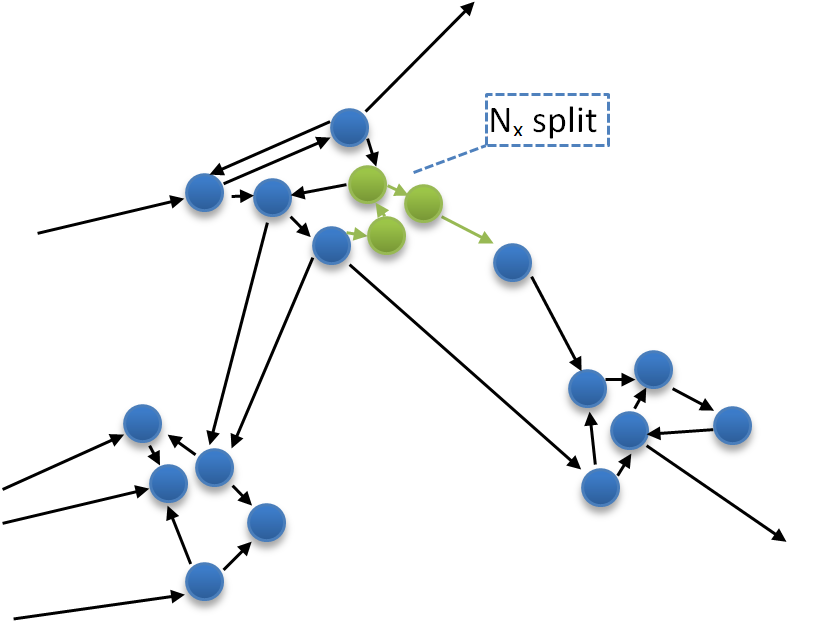
\includegraphics[width=\textwidth]{Figs/likelyEvolution.png}
		\caption{A more likely change scenario in which one part is split into three but where the overall shape of the network is not appreciably altered.}
		\label{fig:likelyEvolution}
	\end{subfigure}
	\begin{subfigure}[t]{0.49\textwidth}
		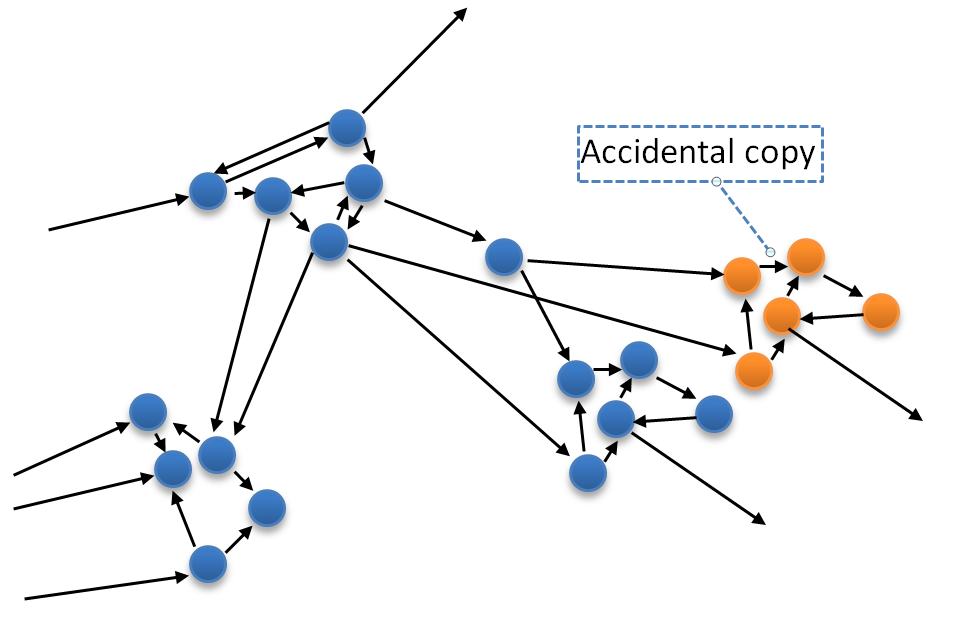
\includegraphics[width=\textwidth]{Figs/copyEvolution.png}
		\caption{A second change scenario in which an entire component is accidentally copied. While the resultant change is large, a small genetic mutation can cause it.}
		\label{fig:copyEvolution}
	\end{subfigure}
	\caption{Means of change in neural networks.}
\end{figure}

\paragraph{Sloman's brain.} One might ask what the relationship between the gradual growth of neural bundles and the observed, large-scale functions in the brain is. We have now supposed at some length that the organisation is not neat, but the question remains whether we can speak of an organisation at all (even a messy one). In {\em Beyond shallow models of emotion} \cite[p. 8]{sloman2000}, Sloman illustrates the possible chaotic organisation of brain with Figure~\ref{fig:slomanBrain}, conjecturing that it might be a jumble of parts that just happen to work together:

\begin{emquote}
	Any observed behaviour might be produced by an unintelligibly tangled and non-modular architecture. (Rectangles represent information stores and buffers, ovals represent processing
	units, and arrows represent flow of information, including control signals.)
\end{emquote}

\begin{figure}
	\centering
	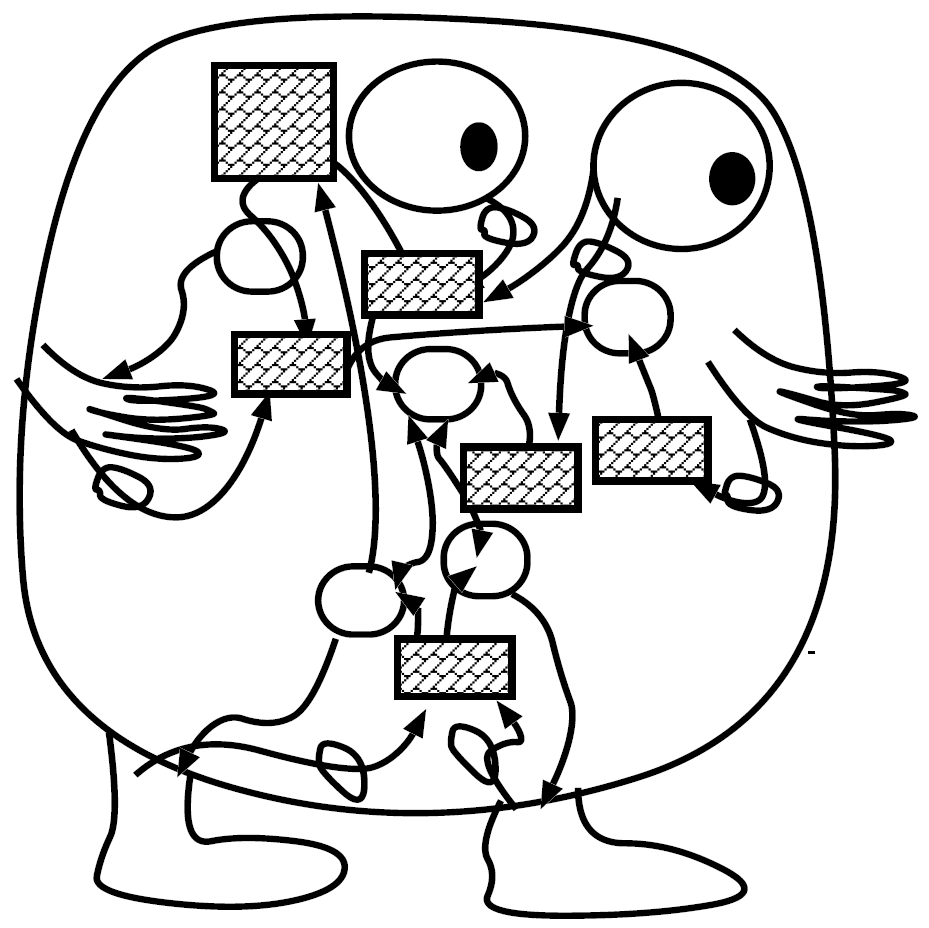
\includegraphics[width=0.6\textwidth]{Figs/slomanBrain.png}
	\caption{Sloman's illustration of the brain as an ``unstructured mess''.}
	\label{fig:slomanBrain}
\end{figure}

This strikes me as a cheery optimism, if anything; one that presupposes that there even are such things as information stores and control signals. The actual situation is, in all likelihood, a far worse one: it is not just different programs that are run in the brain, but entire different models of computation, with the same pattern of activity being interpreted simultaneously in more than one way.
Today, we can scarcely imagine how such an ``architecture'' would work, let alone how one would program --- but if we really want to create genuinely animal intelligences, we will have to find out. Sloman himself admits to the difficulty of gaining understanding of the workings in {\em What Sort of Control System Is Able to Have a Personality?} \cite[p. 6, Section 9 ``Is the task too hard?'']{sloman1997}:
\begin{emquote}
Given the enormous diversity in both design space and niche space and our limited understanding of both, one reaction is extreme pessimism regarding our ability to gain significant insights.
\end{emquote}
The following remedy is offered:
\begin{emquote}
My own attitude is cautious optimism: let us approach the study from many different directions and with many different methodologies and see what we can learn. (\dots)\\
In particular, the Cognition and Affect group at Birmingham has been trying to use a combination of philosophical analysis, critical reflection on shared common sense knowledge about human capabilities, analysis of strength and especially weaknesses in current AI systems, and where appropriate hints from biology, psychology, psychiatry and brain science, to guide a combination of speculation and exploratory implementation (\dots).
\end{emquote}

The methods listed all have their applications, but computational analysis is missing among them. When we talk of psychology, philosophy, and critical reflection, we have already supposed too much; we want to replicate the high-level output of the brain without having explored the mechanism that produces it. In a manner of speaking, we have seen the forest, but do not understand what trees are. If we are to gain the sort of knowledge of brains that we can implement into an AI, we must, empirically, find out about their method of computation. Barring that, we must at least approximate it as far as is practical, and accept that the result will necessarily be an inferior simulacrum.

What, then, is the computational model used in the brain? As yet, nobody knows, and that will stay that way for the foreseeable future. It is very much a guess, but from the concept of slowly growing neural networks (seen in Figures~\ref{fig:neuralNetwork}-\ref{fig:copyEvolution}), one might infer something like the ``active symbol'' hypothesis in Douglas Hofstadter's {\em G\"{o}del Escher Bach}: that patterns of activity form little programs and pieces of data at once; that manipulate other patterns of activation and are manipulated yet other patterns during their lifetime. These are only imperfect analogies, of course. On the coming pages, I shall outline a conceptually compatible white-box model of computation as another, imperfect analogy that will serve as the basis for the model in Sections~\ref{sec:schemaOfCognition}-\ref{sec:mathematicalModel}, and for the implementation of the toy agents in Section-\ref{sec:implementation}.

\section{The Brain as a Collection of White Boxes}\label{sec:whiteBoxModel1}

We now leave the realm of established fact and venture into conjecture. What has been said up to this point has been good, general fact, but it does not suffice for building actual programs. Data on the computational structure of the brain is scarce, thus I will limit myself to positing general, plausible hypotheses about what sorts of structures and loci of computation could have plausibly arisen in it over the course of its evolution. 

A plausible case has been made by Minsky, Sloman, and others (especially in {\em The Emotion Machine} \cite{emotionMachine}) that the brain must possess components in some form. Were it not so, the organ would have long ago succumbed to the innefficiences of its design. As more and more functions are grafted onto a system, the number of interactions between its parts or regions, and therefore the bugs in it, increases. Worse yet, the system becomes brittle: even if, like in a neural network, some accidentally working configuration would have been able to be reached, small changes would surely have upset it again. The part-less system is an evolutionary dead-end from which no improvement is possible, and given how far along our cognition is, it is quite clear that we are not dealing such when we look at our brains.

If we concede that we are dealing with identifiable parts, a second question arises: how do these parts communicate? I would like to deal with with this question in some detail. In the literature, this issue is often glossed over --- in diagrams, one frequently finds unannotated arrows going between functions; the accompanying texts mention concepts like ``selection'', ''message'', and ``sending'' under the implicit assumption that these are merely primitives in no need of further explanation. When we consider the workings of neurons, however, it is not at all clear how groups of them could put together any sort of complex message, and, once put together, how it would travel, and how another group of neurons could receive and interpret it. Are there dedicated interpreters, akin to compilers and runtimes in computer systems? This is not known. I cautiously propose that it is not so, but we can present plausibly-sounding scenarios for both outcomes:
\begin{itemize}
	\item On the one hand, we may image that, early on, some simple message format developed through, allowing more efficient communication between not quite differentiated regions of a nervous system. Over time, this was extended as more components came into play; these new components would have found it easier to make use of the pre-existing protocol. Larger clusters of parts might have even repeated the process and developed simple, internal message formats for communication among themselves. As an orthogonal development, newly developed components might have performed more abstract duties, using older ones as subsidiaries, if at all. To solve conflicts whenever these new and old parts proposed different solutions to whatever issue the organism faced, some other component could have received inputs from both, and adjudicated. In such way, a hierarchical and layered structure could have come into being --- different layers working at different levels of abstraction, and each component only communicating on an on-basis with others. All in all, the whole system would come to resemble a human-developed program.
	
	\item On the other hand, we could imagine quite a different scenario: suppose that the basic scheme of neurons sitting as growths on the communication lines between components never changed. Their basic task was the modulation of signals, and if some new function was to be grafted into the system, then this would have been achieved by growing more neurons that modulated the signals of their fellow neurons. They would not have opened a communication channel with the existing components, but would have listened in on their activity in the manner of interlopers surreptitiously modifying messages. Since neurons would have had no reason to hide their activity (as a black box does), this would have been quite easy and straightforward to do. New bundles of functionality could have inserted themselves into the middle of the information flow (enhancing existing functionality, or adding administrative features), before it (providing pre-processing), or after it (providing post-processing, or usage of the output for higher-level tasks). In contrast to above, we concentrate on the {\em process} of software development instead of its product: a human programmer adds functions one at a time, here and there, extending and refining functionality where fancy strikes or necessity requires.
\end{itemize}

One could thus call the first scenario the \caps{product-oriented view} and the second the \caps{ process-oriented view}: the first looks at the end product of a development, the second posits that the very process of that development, fossilized, is present in the end product.

Evidence is scarce and equivocal for both. In fact, it need not even be the case that they form a dichotomy: we might just as well speculate, for instance, that the second is the low-level reality, but that the first emerged from over time due to the efficiency of its design. The components could be fuzzy, to some degree. We could also posit that the first one ``degenerated'' into the second one; that a formal system is emulating an informal one because of the latter's greater versatility and dynamism.

For the rest of the thesis, I will explore the second of the above two hypotheses, not necessarily because I firmly believe it to be true, but rather because the first one has been tried for some time, and has so far not produced a general AI.

\paragraph{Practical abstraction.} While such a white-box model, and the hypothesizing that preceded it, are conceptually useful, a mesh of gradually grown patterns does not lend itself to implementation in a program. We do not have the capability of faithfully pouring the structure of the human brain into a computerized mould just yet, but, for the time being, we may opt for the next best thing and take cues from it in the hopes of improving our imitations.

\begin{figure}
	\centering
	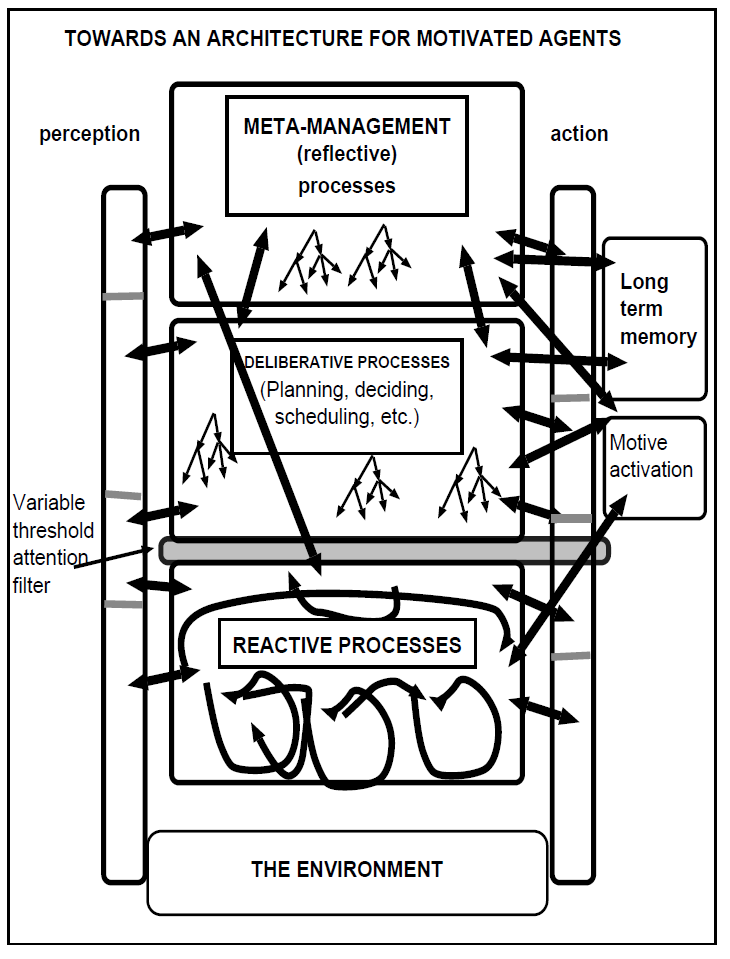
\includegraphics[width=0.8\textwidth]{Figs/slomanSystem.png}
	\caption{Architecture for motivated agents. From \cite[p. 10]{sloman1997}}
	\label{fig:slomanSystem}
\end{figure}

Therefore, I will present a simplified model which, while attempting to remain true to the conceptual view, will, pragmatically, contain discrete functions and components. The white-box nature of brain activity will be emulated by a message-passing scheme in which messages model the internal activity of components. Instead of each component blindly acting in some fashion on the activity of another, components will have explicit parsers and interpreters and later, these will be further simplified into localized message formats and tagging, for the sake of easy implementation.
This effort is guided by the same thought as Sloman's cognitive architecture see in Figure~\ref{fig:slomanSystem}. It is not a truly accurate representation of the brain and it does not claim to be, but it is {\em something like it}; something that is close, and good, enough. We will meet this cognitive architecture again later, but for now, we move on to the description of neural components.

%While some form interpretation surely must happen in one or more places, it is implausible to suppose that there is one agreed-upon message format, or one programming language that all parts use. 
%
%
%The facts and processes of the previous subsection are relatively uncontroversial and can be found reiterated in any textbook on the evolution of nervous systems. The functional structure and the model of computation used in the brain, however, are not well understood. FMRI and similar brain imagining techniques, while invaluable, give only rough impressions about the neural correlates of certain forms of cognition and do not give fine-grained insight into its structure. As such, the model I shall describe in the following paragraphs is a conjecture. The implication of such an evolutionary viewpoint, I conjecture in this document, is that brain functions don't ``just appear'', but are rather the result of small changes and the recombination of pre-existing parts. This, in turn, informs the plausibility of various possible brain architectures. It becomes unlikely that the brain should be a collection of neatly delineated functions, or that it should have certain coordinating units or universal message formats for communication between components. The reason for this is that administrative mechanism confer little evolutionary benefit on their own, and do not confer it gradually: the imposition of a central coordinating mechanism on a pre-existing mesh of neurons would necessitate the complete reorganisation of such, and the abandonment of the previous communication channels in favour centralized coordination. The same objections can be raised against a universal or even a local message format. Moreover, such mechanisms require substantial changes in the organism with no obvious or immediate advantage.
%
%These objections do not contradict the existence of macroscopic structures in the brain, dedicated to certain tasks. The development and adaptation of such remains entirely plausible. They do, however, give insight into the pattern of processing inside such structures, which is often simply regarded as atomic or replicated in computers as if it were a conventional engineering product.
%
%Instead of a rigidly ordered brain with central organisation and large, discrete, and highly complex features like ``sight'' or ``reason'' which function like ready-made black boxes, to be plugged in at will, I propose a decentralized white-box architecture composed of simple parts: first, every component, while perhaps sophisticated, is conceptually simple. Second, communication between different components is not performed in the function-call pattern of computer programs, but rather by one component listening in on the activity of another. Since there is, inherently, no mechanism of function abstraction in neural systems, it stands to reason that the most likely way for new functions to develop is for additional neurons to modulate the activity of others. In such a scheme, a visual perception component does not have to know which other components will consume its output (or rather, listen on its activity); changes which affect agent activity in useful ways based on the visual data can occur gradually and, over time, become large enough to count as components in their own right.
